\chapter{Análise Estatística Não Paramétrica}
\label{chap:analise_estatistica_np}

Tendo em vista que os dados das métricas de conectividade (diferença entre Pós e Pré) não se comportam de maneira normal (ver Capítulo~\ref{chap:analise_distribuicao_normalidade}), optamos por empregar testes estatísticos não paramétricos para comparar as condições de estimulação (\texorpdfstring{\textit{cathodic} versus \textit{sham}}{cathodic versus sham}). Essa escolha evita pressupostos inadequados sobre a distribuição dos dados e confere maior robustez às inferências.

Nesta etapa, foram aplicados os seguintes testes:
\begin{itemize}
    \item \textbf{Mann-Whitney U:} Teste para amostras independentes, comparando as condições para cada faixa de frequência e grupo de canais. O efeito foi estimado pela fórmula:
    \[
    \text{effect size} = \frac{2\cdot \text{stat}}{n_{\text{cathodic}} \cdot n_{\text{sham}}} - 1.
    \]
    \item \textbf{Wilcoxon:} Teste para amostras pareadas, no qual os dados foram emparelhados por atleta, par de canais e faixa de frequência, possibilitando uma comparação intraindividual entre as condições.
    \item \textbf{Kruskal-Wallis:} Teste para múltiplos grupos, empregado para comparar as condições quando os dados foram agrupados por faixa de frequência, com o tamanho do efeito estimado pela razão entre a estatística do teste e o número total de observações menos um.
\end{itemize}

Os testes foram realizados separadamente para cada uma das métricas de conectividade:
\begin{itemize}
    \item \texorpdfstring{\texttt{median\_plv\_diff}}{median_plv_diff}
    \item \texorpdfstring{\texttt{median\_pli\_diff}}{median_pli_diff}
    \item \texorpdfstring{\texttt{median\_cf\_plm\_diff}}{median_cf_plm_diff}
\end{itemize}
e para os dois grupos de canais: \texorpdfstring{\texttt{EEG\_EEG}}{EEG_EEG} e \texorpdfstring{\texttt{EEG\_ECG}}{EEG_ECG}. Ressalta-se que, embora o código inclua procedimentos para remoção de dados nulos, na prática esses valores não estão presentes, servindo apenas para tratamento de exceções.

\section{Resultados dos Testes}

\subsection{\texorpdfstring{Métricas para \texttt{median\_plv\_diff}}{Métricas para median\_plv\_diff}}
\paragraph{Grupo EEG\_EEG:}
\begin{itemize}
    \item \textbf{Mann-Whitney U:} As faixas \emph{alpha, beta, delta, gamma} e \emph{theta} apresentaram p-valores extremamente baixos (por exemplo, $p < 10^{-29}$ para \emph{alpha} e $p < 10^{-132}$ para \emph{gamma}), indicando diferenças estatisticamente significativas entre as condições. Os tamanhos de efeito variaram, com valores próximos a $-0.088$ e $0.191$.
    \item \textbf{Wilcoxon:} Os testes pareados mostraram p-valores próximos de zero para todas as faixas, com tamanhos de efeito em torno de $0.393$.
    \item \textbf{Kruskal-Wallis:} Também foram encontradas diferenças significativas em todas as faixas, com tamanhos de efeito entre $0.0058$ e $0.0273$.
\end{itemize}

\paragraph{Grupo EEG\_ECG:}
\begin{itemize}
    \item \textbf{Mann-Whitney U:} Foram significativas as faixas \emph{alpha, beta} e \emph{theta} (p-valores menores que 0.001) e a \emph{gamma} apresentou um p-valor marginal ($p \approx 0.041$), enquanto a faixa \emph{delta} não alcançou significância ($p \approx 0.148$).
    \item \textbf{Wilcoxon:} Os testes demonstraram diferenças robustas, com p-valores extremamente baixos e tamanhos de efeito de aproximadamente $0.381$.
    \item \textbf{Kruskal-Wallis:} Os resultados foram significativos para \emph{alpha, beta} e \emph{theta}, mas não para \emph{delta} e \emph{gamma}.
\end{itemize}

\subsection{\texorpdfstring{Métricas para \texttt{median\_pli\_diff}}{Métricas para median\_pli\_diff}}
\paragraph{Grupo EEG\_EEG:}
\begin{itemize}
    \item \textbf{Mann-Whitney U:} As faixas \emph{alpha, delta, gamma} e \emph{theta} apresentaram diferenças significativas (p-valores $< 0.001$), enquanto a faixa \emph{beta} teve um resultado marginal ($p \approx 0.051$).
    \item \textbf{Wilcoxon:} Os testes pareados indicaram significância robusta em todas as faixas, com tamanho de efeito em torno de $0.477$.
    \item \textbf{Kruskal-Wallis:} As faixas \emph{alpha, delta, gamma} e \emph{theta} foram significativamente diferentes, com \emph{beta} sendo marginalmente não significativo.
\end{itemize}

\paragraph{Grupo EEG\_ECG:}
\begin{itemize}
    \item \textbf{Mann-Whitney U:} Apenas as faixas \emph{delta} e \emph{gamma} mostraram diferenças significativas, enquanto \emph{alpha} e \emph{beta} não atingiram significância.
    \item \textbf{Wilcoxon:} Todos os testes foram altamente significativos, com tamanhos de efeito próximos a $0.441$.
    \item \textbf{Kruskal-Wallis:} Apenas \emph{alpha, delta} e \emph{gamma} foram significativas; as faixas \emph{beta} e \emph{theta} não apresentaram diferenças estatísticas.
\end{itemize}

\subsection{\texorpdfstring{Métricas para \texttt{median\_cf\_plm\_diff}}{Métricas para median\_cf\_plm\_diff}}
\paragraph{Grupo EEG\_EEG:}
\begin{itemize}
    \item \textbf{Mann-Whitney U:} Todas as faixas foram significativamente diferentes entre as condições (p-valores muito baixos), com tamanhos de efeito variando de $-0.062$ a $0.274$.
    \item \textbf{Wilcoxon:} Resultados extremamente significativos foram observados para todas as faixas, com tamanho de efeito em torno de $0.355$.
    \item \textbf{Kruskal-Wallis:} Todas as faixas apresentaram diferenças significativas, com tamanhos de efeito entre $0.0029$ e $0.0563$.
\end{itemize}

\paragraph{Grupo EEG\_ECG:}
\begin{itemize}
    \item \textbf{Mann-Whitney U:} Foram significativas as faixas \emph{alpha, beta} e \emph{delta} (p-valores menores que 0.05), enquanto \emph{gamma} e \emph{theta} não apresentaram significância.
    \item \textbf{Wilcoxon:} Todos os testes resultaram em p-valores extremamente baixos, com tamanhos de efeito de aproximadamente $0.358$.
    \item \textbf{Kruskal-Wallis:} As faixas \emph{alpha, beta} e \emph{gamma} foram significativas, mas \emph{delta} e \emph{theta} não apresentaram diferenças estatísticas.
\end{itemize}

\section{Discussão e Justificativa dos Métodos}

Dado que os testes de normalidade indicaram violações significativas do pressuposto de normalidade para as três métricas analisadas, a utilização de testes não paramétricos se mostrou necessária. Tais métodos não dependem de pressupostos sobre a distribuição dos dados, oferecendo uma análise mais robusta e confiável. Além disso, a aplicação de múltiplos testes (Mann-Whitney U, Wilcoxon e Kruskal-Wallis) permitiu uma avaliação abrangente das diferenças entre as condições \texorpdfstring{\texttt{cathodic}}{cathodic} e \texorpdfstring{\texttt{sham}}{sham}, considerando tanto comparações entre grupos independentes quanto análises pareadas intraindividuais.

Os resultados indicam que, para a maioria das faixas de frequência e para as métricas \texorpdfstring{\texttt{median\_plv\_diff}}{median_plv_diff} e \texorpdfstring{\texttt{median\_cf\_plm\_diff}}{median_cf_plm_diff}, existem diferenças estatisticamente significativas entre as condições, reforçando a importância da modulação induzida pela estimulação. Por sua vez, os achados para \texorpdfstring{\texttt{median\_pli\_diff}}{median_pli_diff} foram menos consistentes, variando conforme o teste e a faixa considerada.

Em suma, a escolha dos testes não paramétricos foi justificada pela distribuição não normal dos dados, e os resultados obtidos fornecem evidências sólidas de diferenças na sincronização de fase entre as condições experimentais, reforçando os efeitos da estimulação no contexto das análises de conectividade.

\section{Detecção de Outliers, Análise Bootstrap e Correções para Comparações Múltiplas}

Para aprimorar a qualidade dos dados e reduzir o impacto de pontos atípicos nas análises subsequentes, executamos uma etapa de detecção e remoção de outliers utilizando o método ECOD (Empirical Cumulative Distribution-based Outlier Detection). Esse método é especialmente adequado para nosso conjunto de dados por sua natureza não paramétrica, que permite identificar anomalias sem pressupor uma distribuição específica. O ECOD estima a função de distribuição cumulativa empírica em cada dimensão, identificando como outliers os pontos que se desviam significativamente do comportamento esperado. Estudos demonstram que essa abordagem supera diversas técnicas de detecção de outliers em termos de acurácia e eficiência \cite{li2022}.

Aplicamos o ECOD considerando as métricas \texorpdfstring{\texttt{median\_plv\_diff}}{median_plv_diff}, \texorpdfstring{\texttt{median\_pli\_diff}}{median_pli_diff} e \texorpdfstring{\texttt{median\_cf\_plm\_diff}}{median_cf_plm_diff}. Inicialmente, o dataset continha 122915 entradas; após a aplicação do ECOD, identificamos 6146 outliers, o que corresponde a aproximadamente 5.00\% dos dados. A remoção desses outliers resultou em um dataset com 116769 linhas, melhorando a confiabilidade das análises posteriores.

Posteriormente, implementamos um robusto pipeline de análise por meio de bootstrap acelerado por GPU, utilizando CuPy para calcular intervalos de confiança BCa (Bias-Corrected and Accelerated). Esse método é particularmente robusto, pois ajusta tanto o viés quanto a aceleração da distribuição bootstrap, permitindo capturar as assimetrias e a presença de outliers nos dados. Essa abordagem, embora computacionalmente custosa, é amplamente considerada uma das mais robustas para a estimação de intervalos de confiança em situações em que os pressupostos de normalidade não são atendidos. Além disso, o método BCa foi escolhido em detrimento de outros métodos de intervalo de confiança por sua capacidade de corrigir a distorção na distribuição da estatística estimada.

A análise é realizada agrupando os dados por combinações de \emph{channel pair}, \emph{frequency band} e \emph{channel group} (os quais são mutuamente exclusivos, como \texorpdfstring{\texttt{EEG\_EEG}}{EEG_EEG} e \texorpdfstring{\texttt{EEG\_ECG}}{EEG_ECG}). Essa estratégia permite comparar diferenças entre as condições dentro de cada subgrupo. Para mitigar o risco de falsos positivos decorrentes do elevado número de comparações (estimado em 11346 testes, considerando 1891 channel pairs e 6 faixas de frequência), foram aplicadas correções para comparações múltiplas. Entre os métodos de correção, o Bonferroni se destaca por sua extrema rigidez e conservadorismo, sendo considerado o mais robusto, principalmente em contextos com um elevado número de testes. Embora métodos como Holm e FDR-BH também tenham sido calculados e estejam disponíveis para comparação, o Bonferroni é adotado como referência primária na decisão de significância, visto que o threshold ajustado (aproximadamente 0.00000441) minimiza o risco de erros do tipo I.

Além disso, em nosso pipeline também foram computados tamanhos de efeito utilizando diversas métricas, tais como:
\begin{itemize}
    \item \textbf{Cohen's d} e \textbf{Hedges' g}: que quantificam a magnitude da diferença entre as condições em termos de desvios-padrão;
    \item \textbf{Rank-Biserial Correlation (RBC)}: derivado do teste de Wilcoxon, que fornece uma interpretação robusta baseada em postos.
\end{itemize}
Essas métricas complementares permitem uma avaliação abrangente do efeito da estimulação e possibilitam a comparação dos resultados com os intervalos de confiança BCa e os valores-p corrigidos pelo método Bonferroni. Na tabela de resultados em anexo, os leitores encontrarão também as correções de Holm e FDR-BH, bem como os tamanhos de efeito calculados, permitindo uma comparação completa dos diferentes métodos.

Em resumo, nossa abordagem compreende as seguintes etapas:
\begin{enumerate}
    \item \textbf{Detecção de Outliers:} Utilizamos o ECOD para identificar e remover aproximadamente 5\% dos dados que se comportavam como anomalias, garantindo a robustez dos dados para análise.
    \item \textbf{Análise Bootstrap com GPU:} Implementamos o cálculo de intervalos de confiança BCa, estimando viés, erro padrão e tamanhos de efeito por meio de reamostragem (bootstrap) acelerada por GPU, garantindo a precisão dos intervalos mesmo com distribuições assimétricas.
    \item \textbf{Testes Não Paramétricos e Correção para Comparações Múltiplas:} Aplicamos o teste de Wilcoxon (para dados emparelhados) e outras análises não paramétricas, e corrigimos os valores-p utilizando métodos conservadores, com ênfase no Bonferroni, para reduzir o risco de erros do tipo I.
\end{enumerate}

Os resultados deste processamento serão apresentados em detalhes nos anexos, permitindo a comparação dos resultados obtidos com e sem a remoção de outliers, e a análise dos diferentes tamanhos de efeito e métodos de correção.

\section{Distribuição de Tamanhos de Efeito e p-valores}
\label{sec:effect_size_distribution}

Nesta etapa, examinamos a distribuição das estimativas de tamanho de efeito (\emph{Cohen's d}, \emph{Hedges' g} e \emph{Wilcoxon RBC}) e dos valores-p (brutos e corrigidos por Bonferroni) para as análises de PLI (EEG-EEG) e CF-PLM (EEG-ECG), considerando cenários com e sem outliers. A Figura~\ref{fig:effectsizehist_all} ilustra, em quatro subfiguras, como essas métricas se distribuem ao longo dos pares de canal e faixas de frequência analisados.

\begin{figure}[htb]
    \centering
    % Subfigura 1: PLI (EEG-EEG), Sem Outliers
    \subfloat[Sem Outliers -- PLI (EEG-EEG)]{
        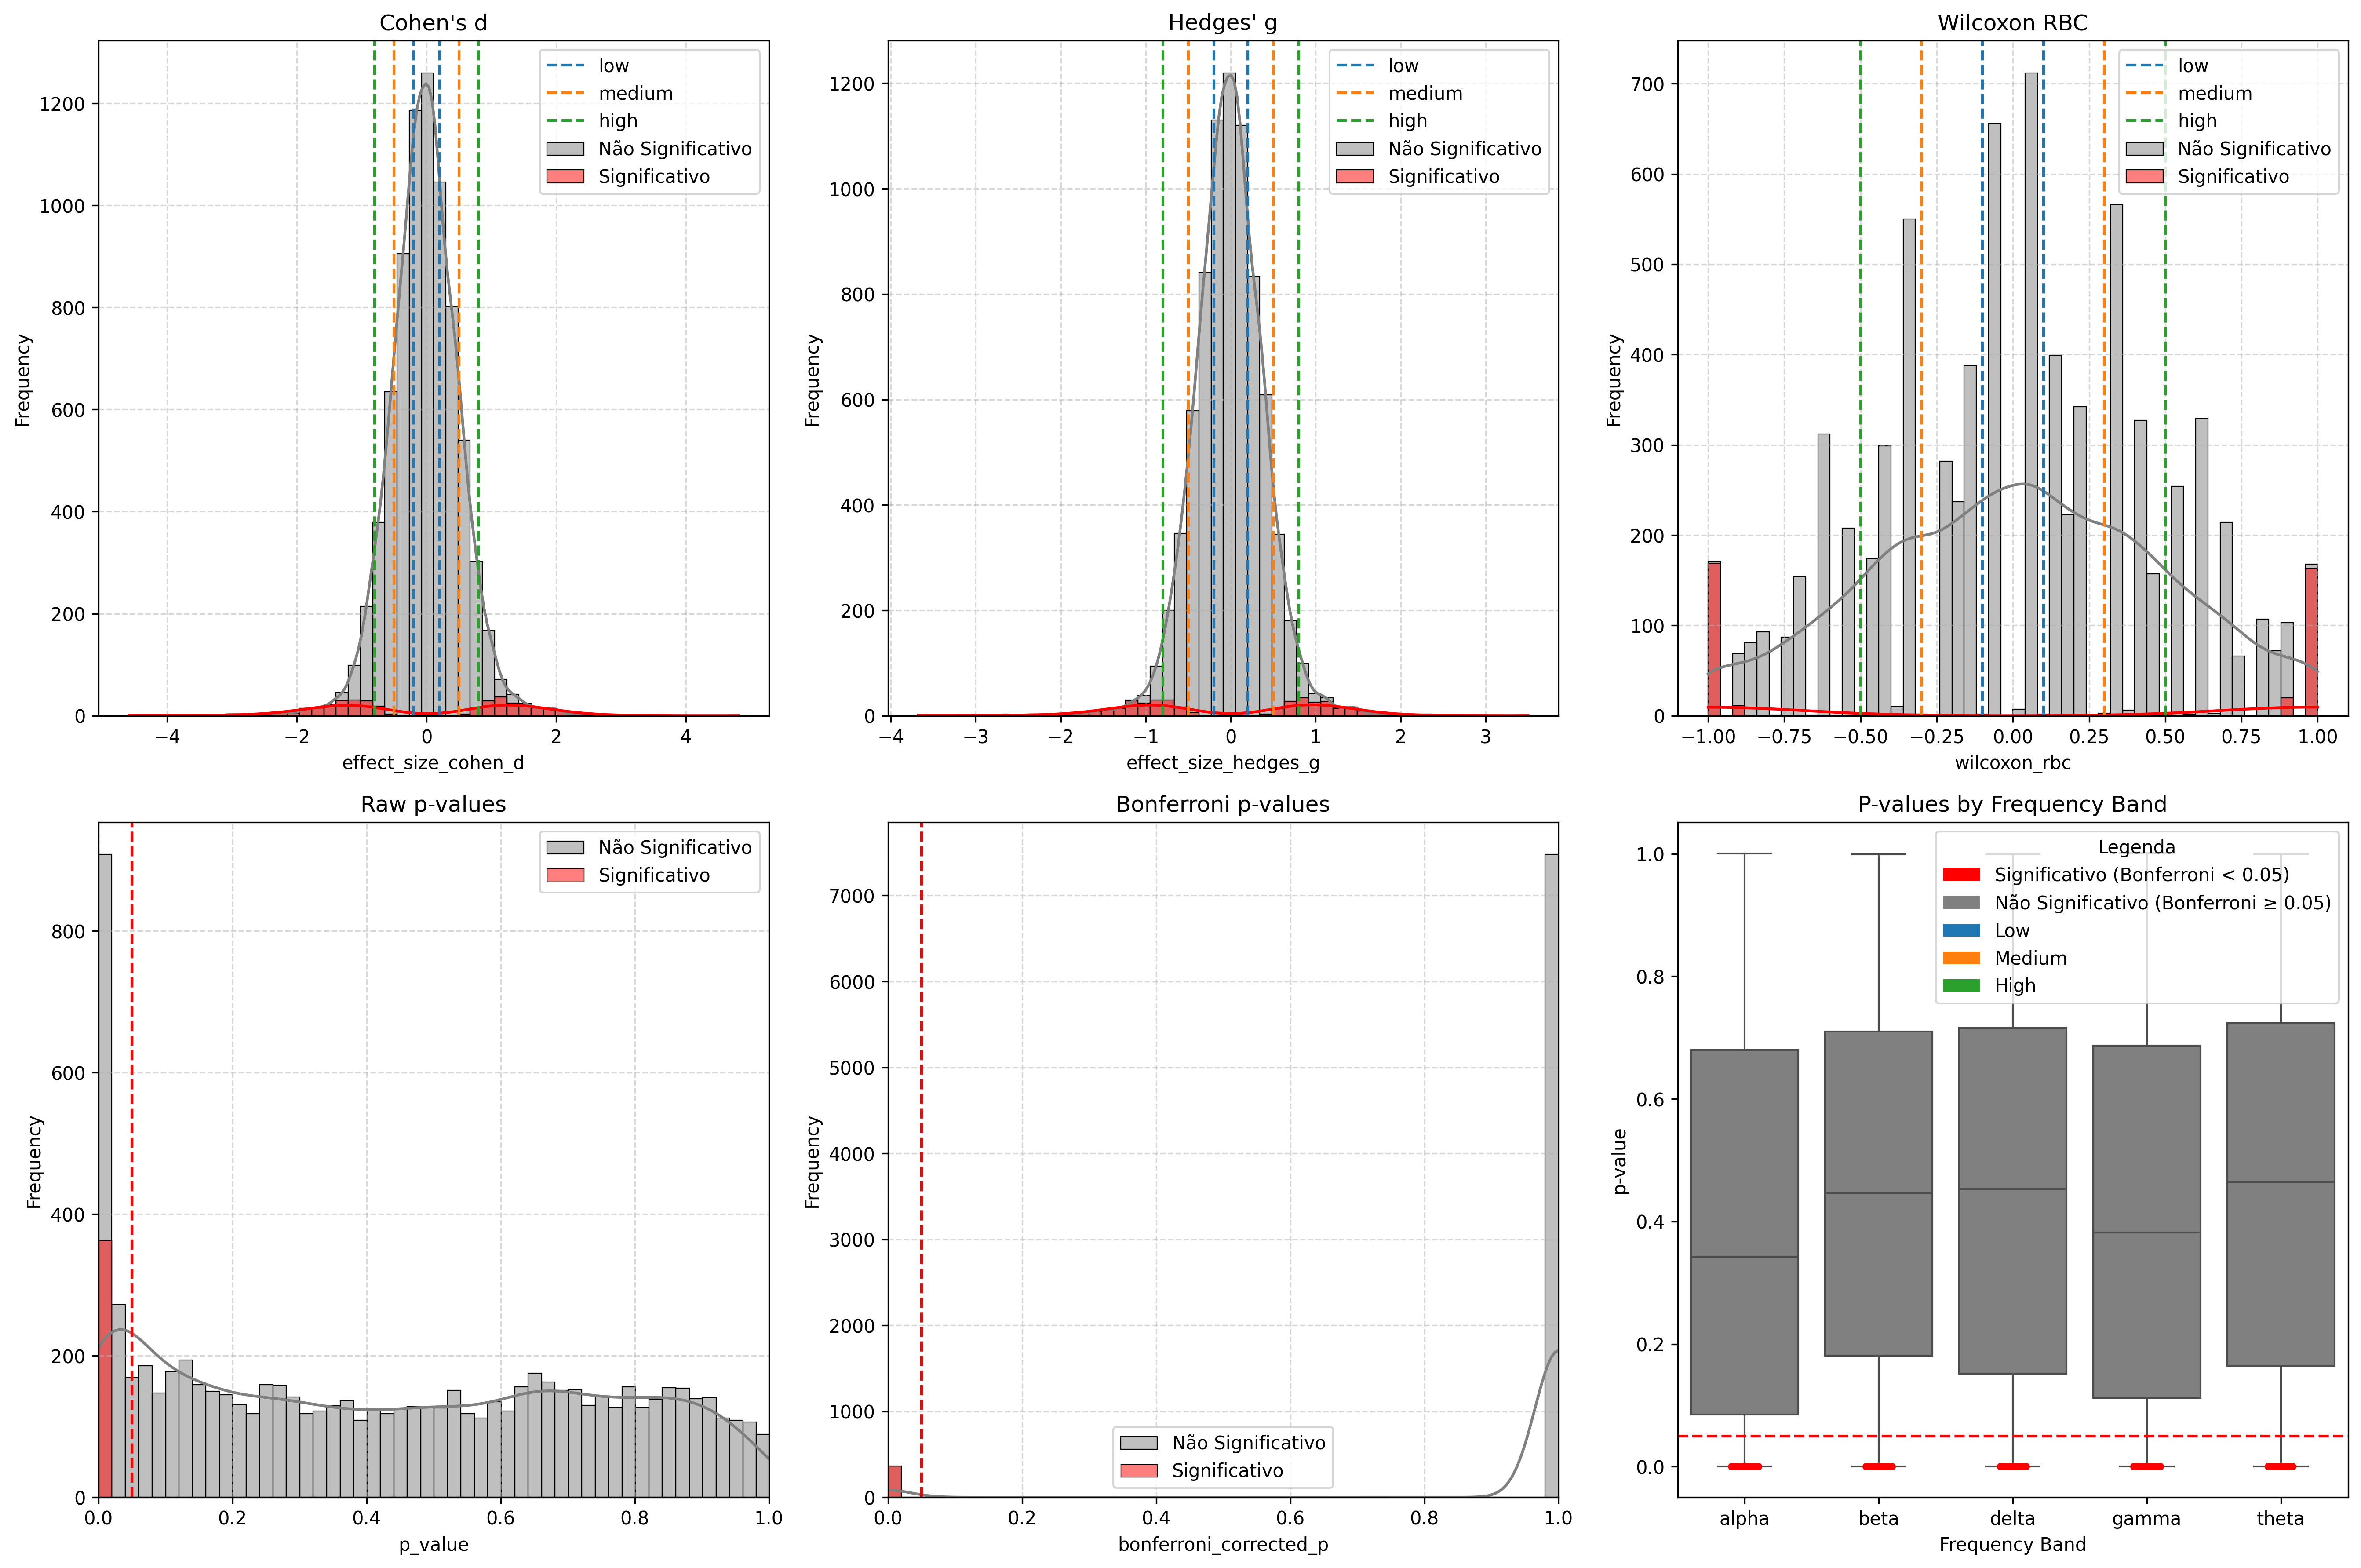
\includegraphics[width=0.45\textwidth]{figs/7_bootstrap_results_analysis/1_effect_size_histograms/Effect_Size_Histograms_PLI_EEGEEG_Sem_Outliers.png}
    }
    \quad
    % Subfigura 2: CF-PLM (EEG-ECG), Sem Outliers
    \subfloat[Sem Outliers -- CF-PLM (EEG-ECG)]{
        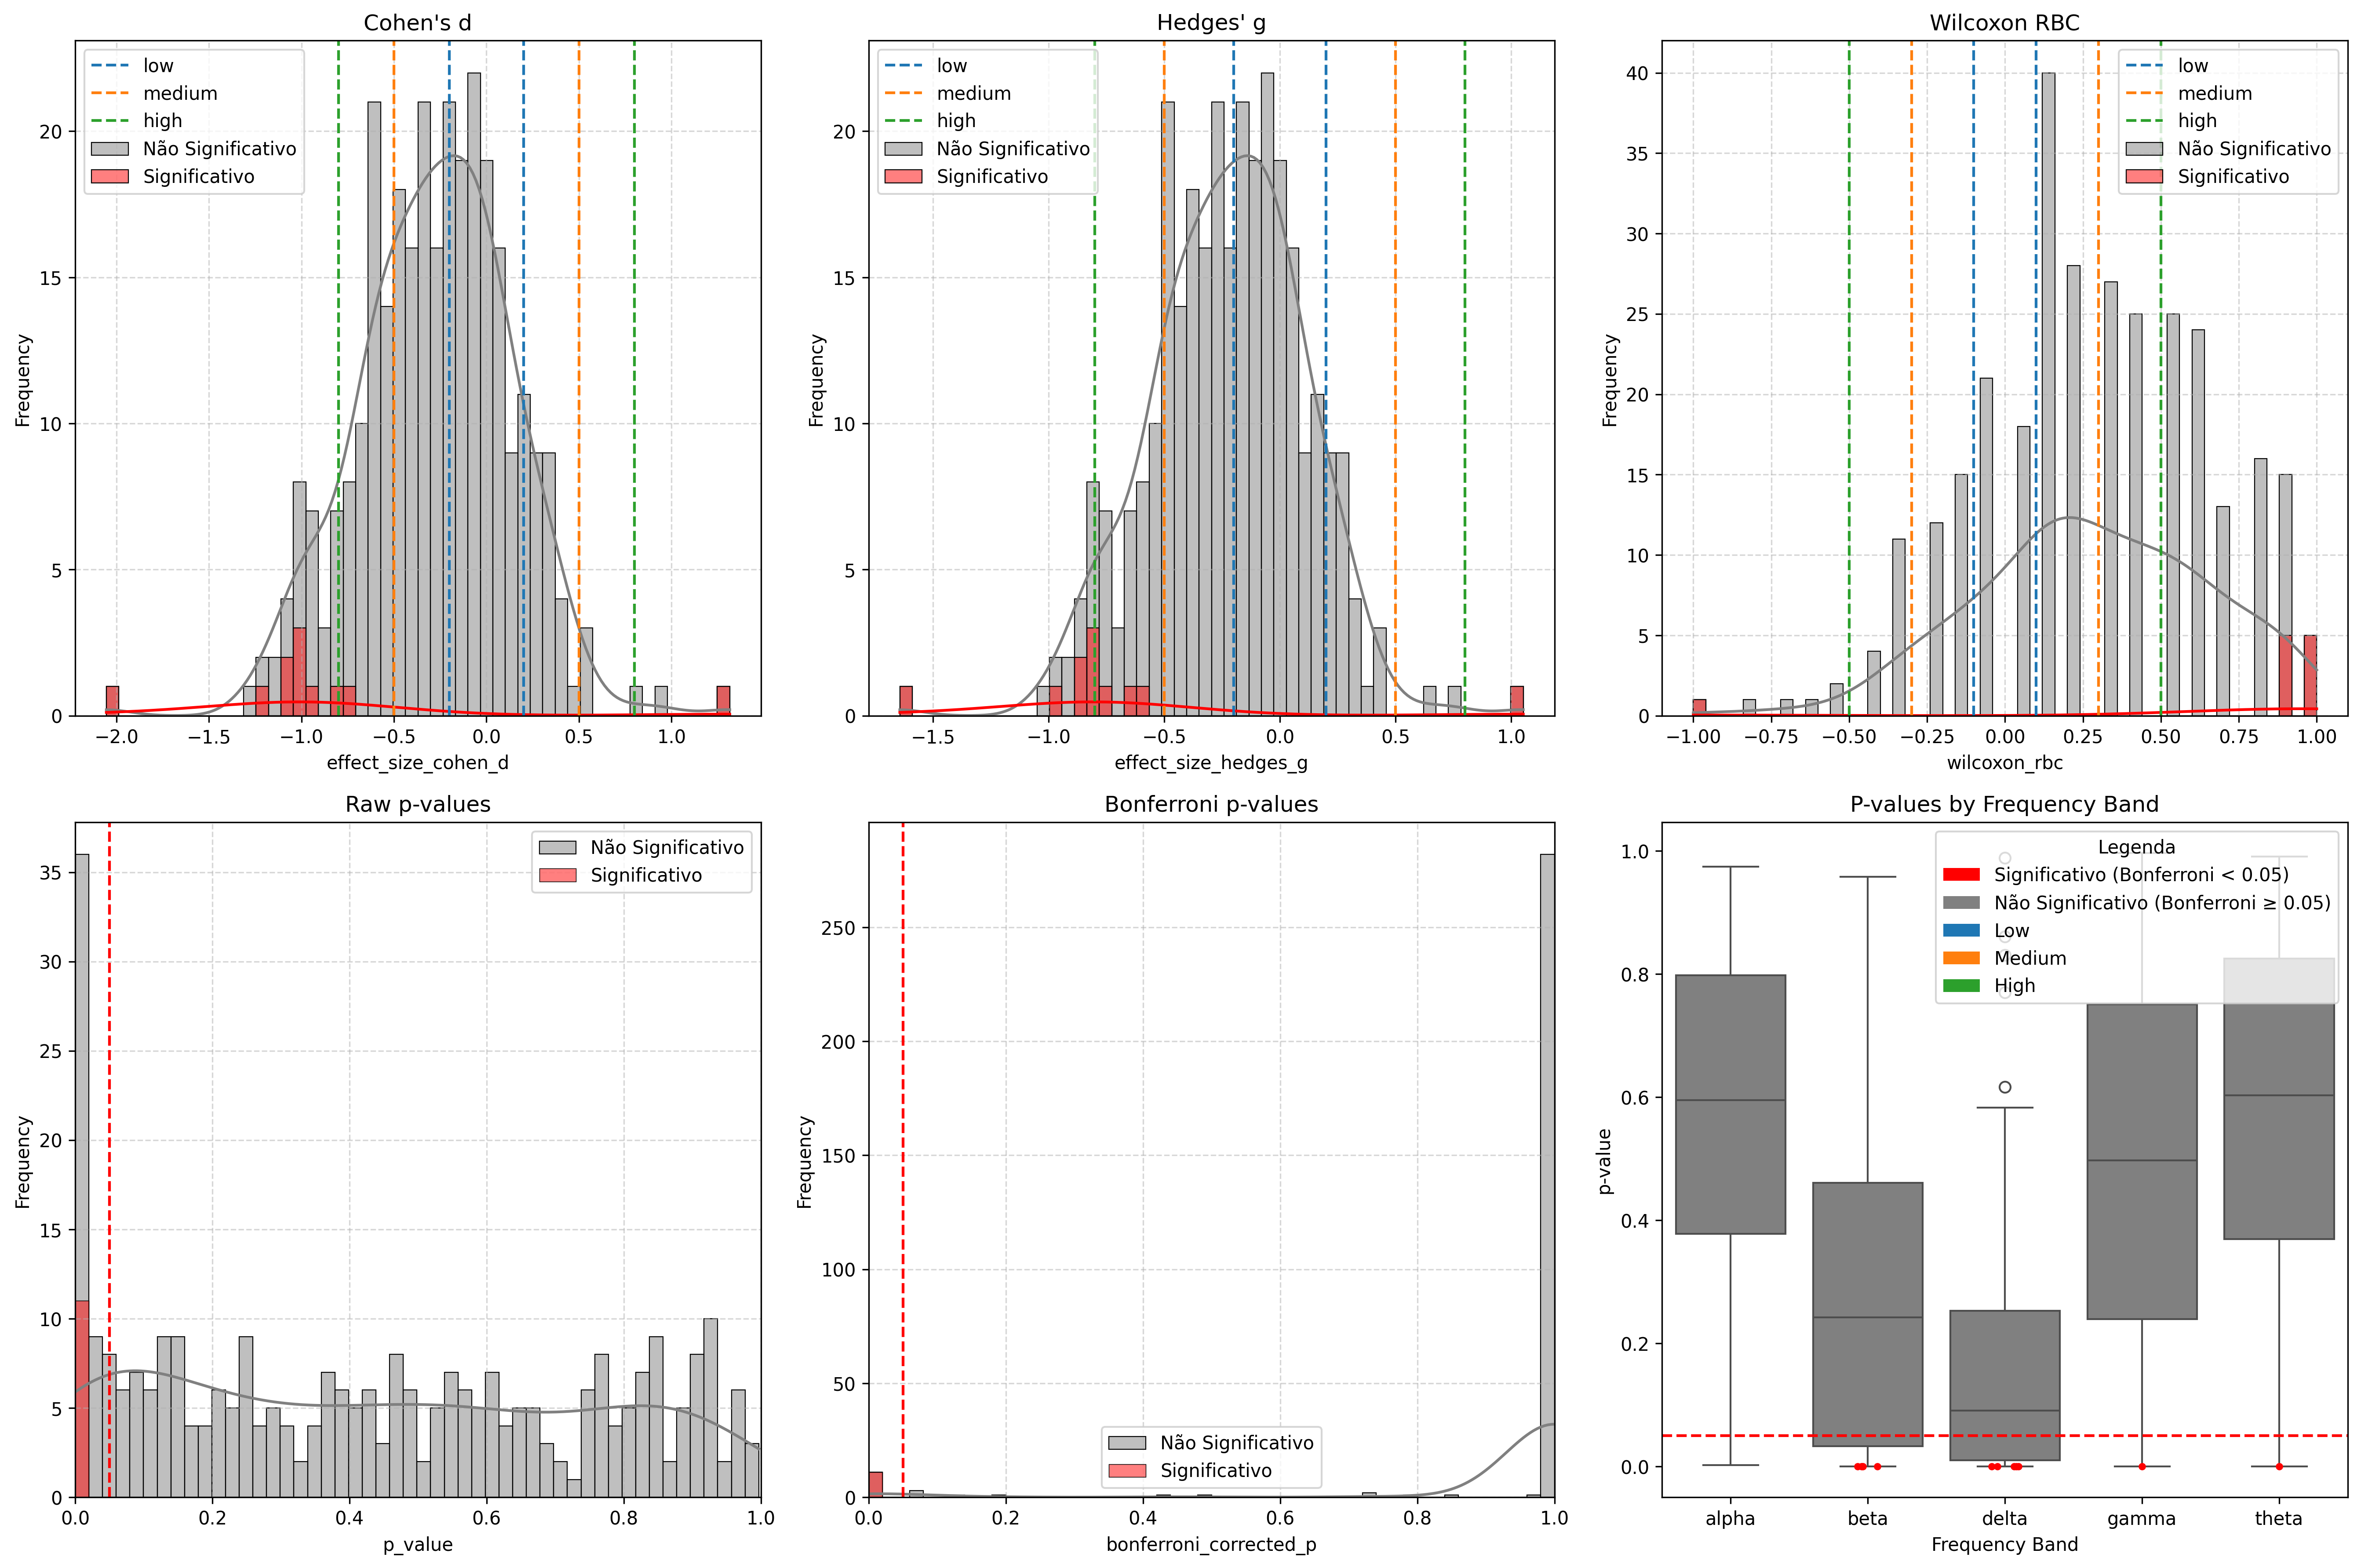
\includegraphics[width=0.45\textwidth]{figs/7_bootstrap_results_analysis/1_effect_size_histograms/Effect_Size_Histograms_CFPLM_EEGECG_Sem_Outliers.png}
    }
    \\
    % Subfigura 3: PLI (EEG-EEG), Com Outliers
    \subfloat[Com Outliers -- PLI (EEG-EEG)]{
        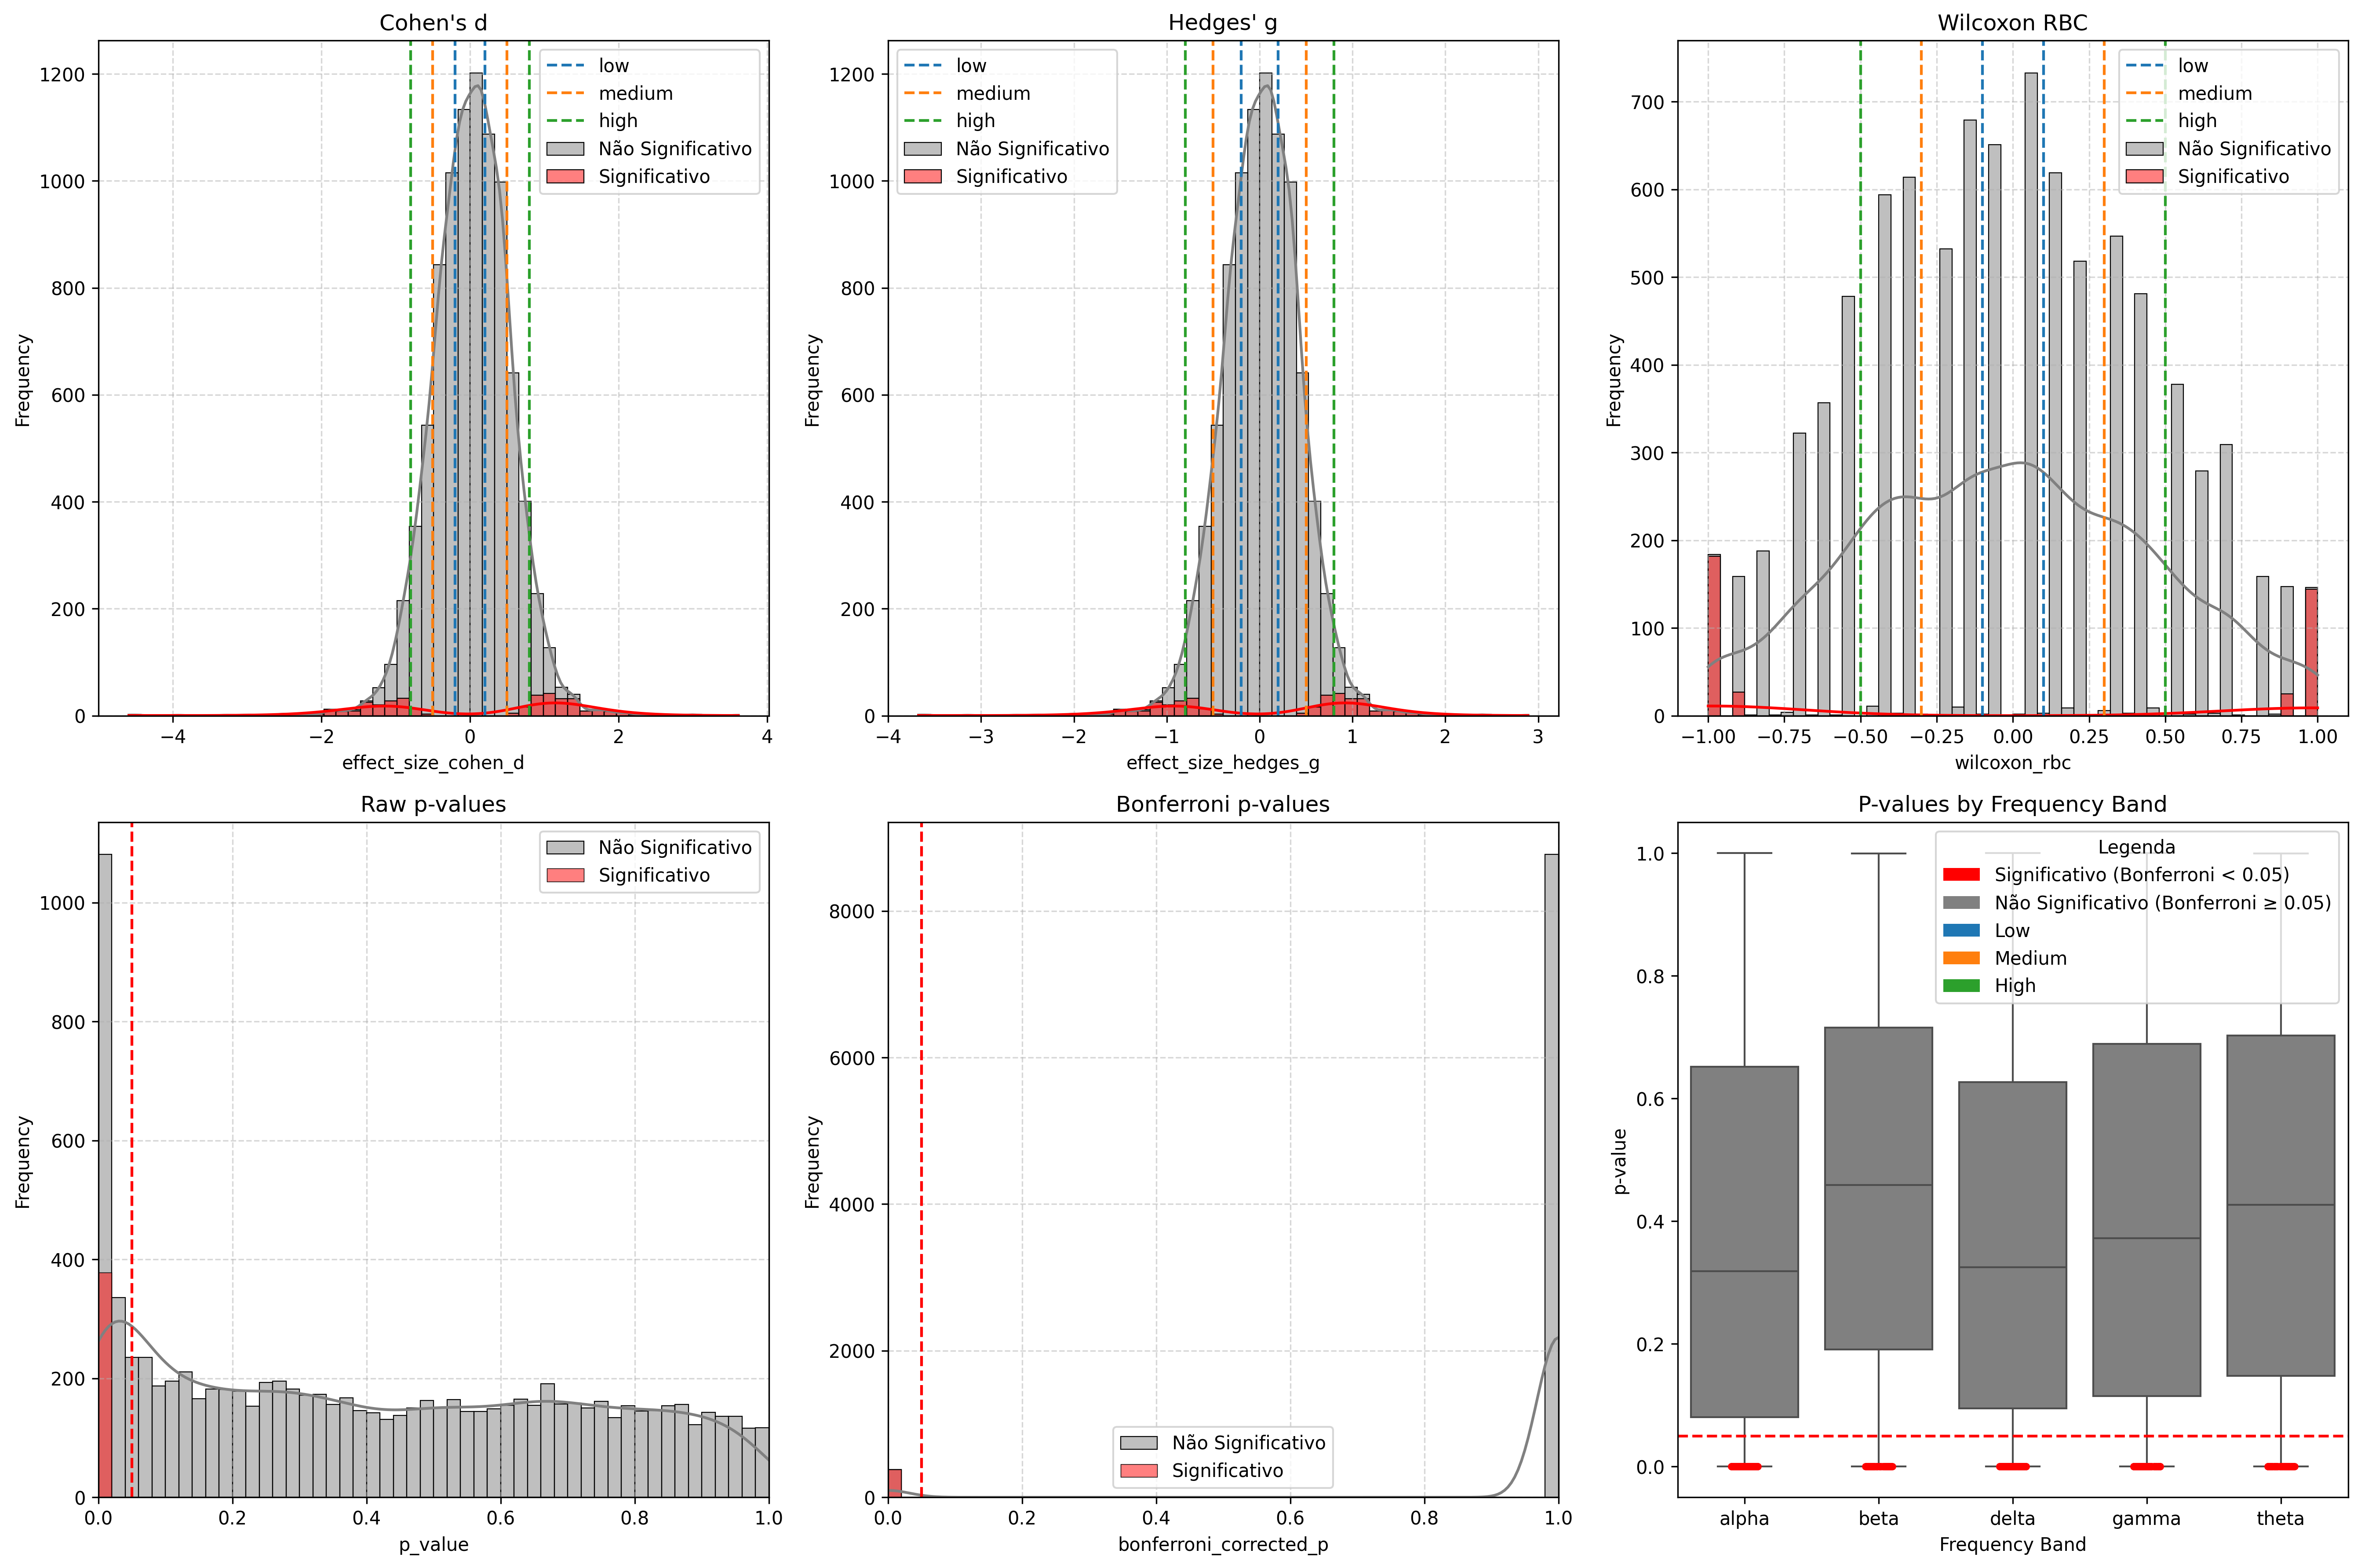
\includegraphics[width=0.45\textwidth]{figs/7_bootstrap_results_analysis/1_effect_size_histograms/Effect_Size_Histograms_PLI_EEGEEG_Com_Outliers.png}
    }
    \quad
    % Subfigura 4: CF-PLM (EEG-ECG), Com Outliers
    \subfloat[Com Outliers -- CF-PLM (EEG-ECG)]{
        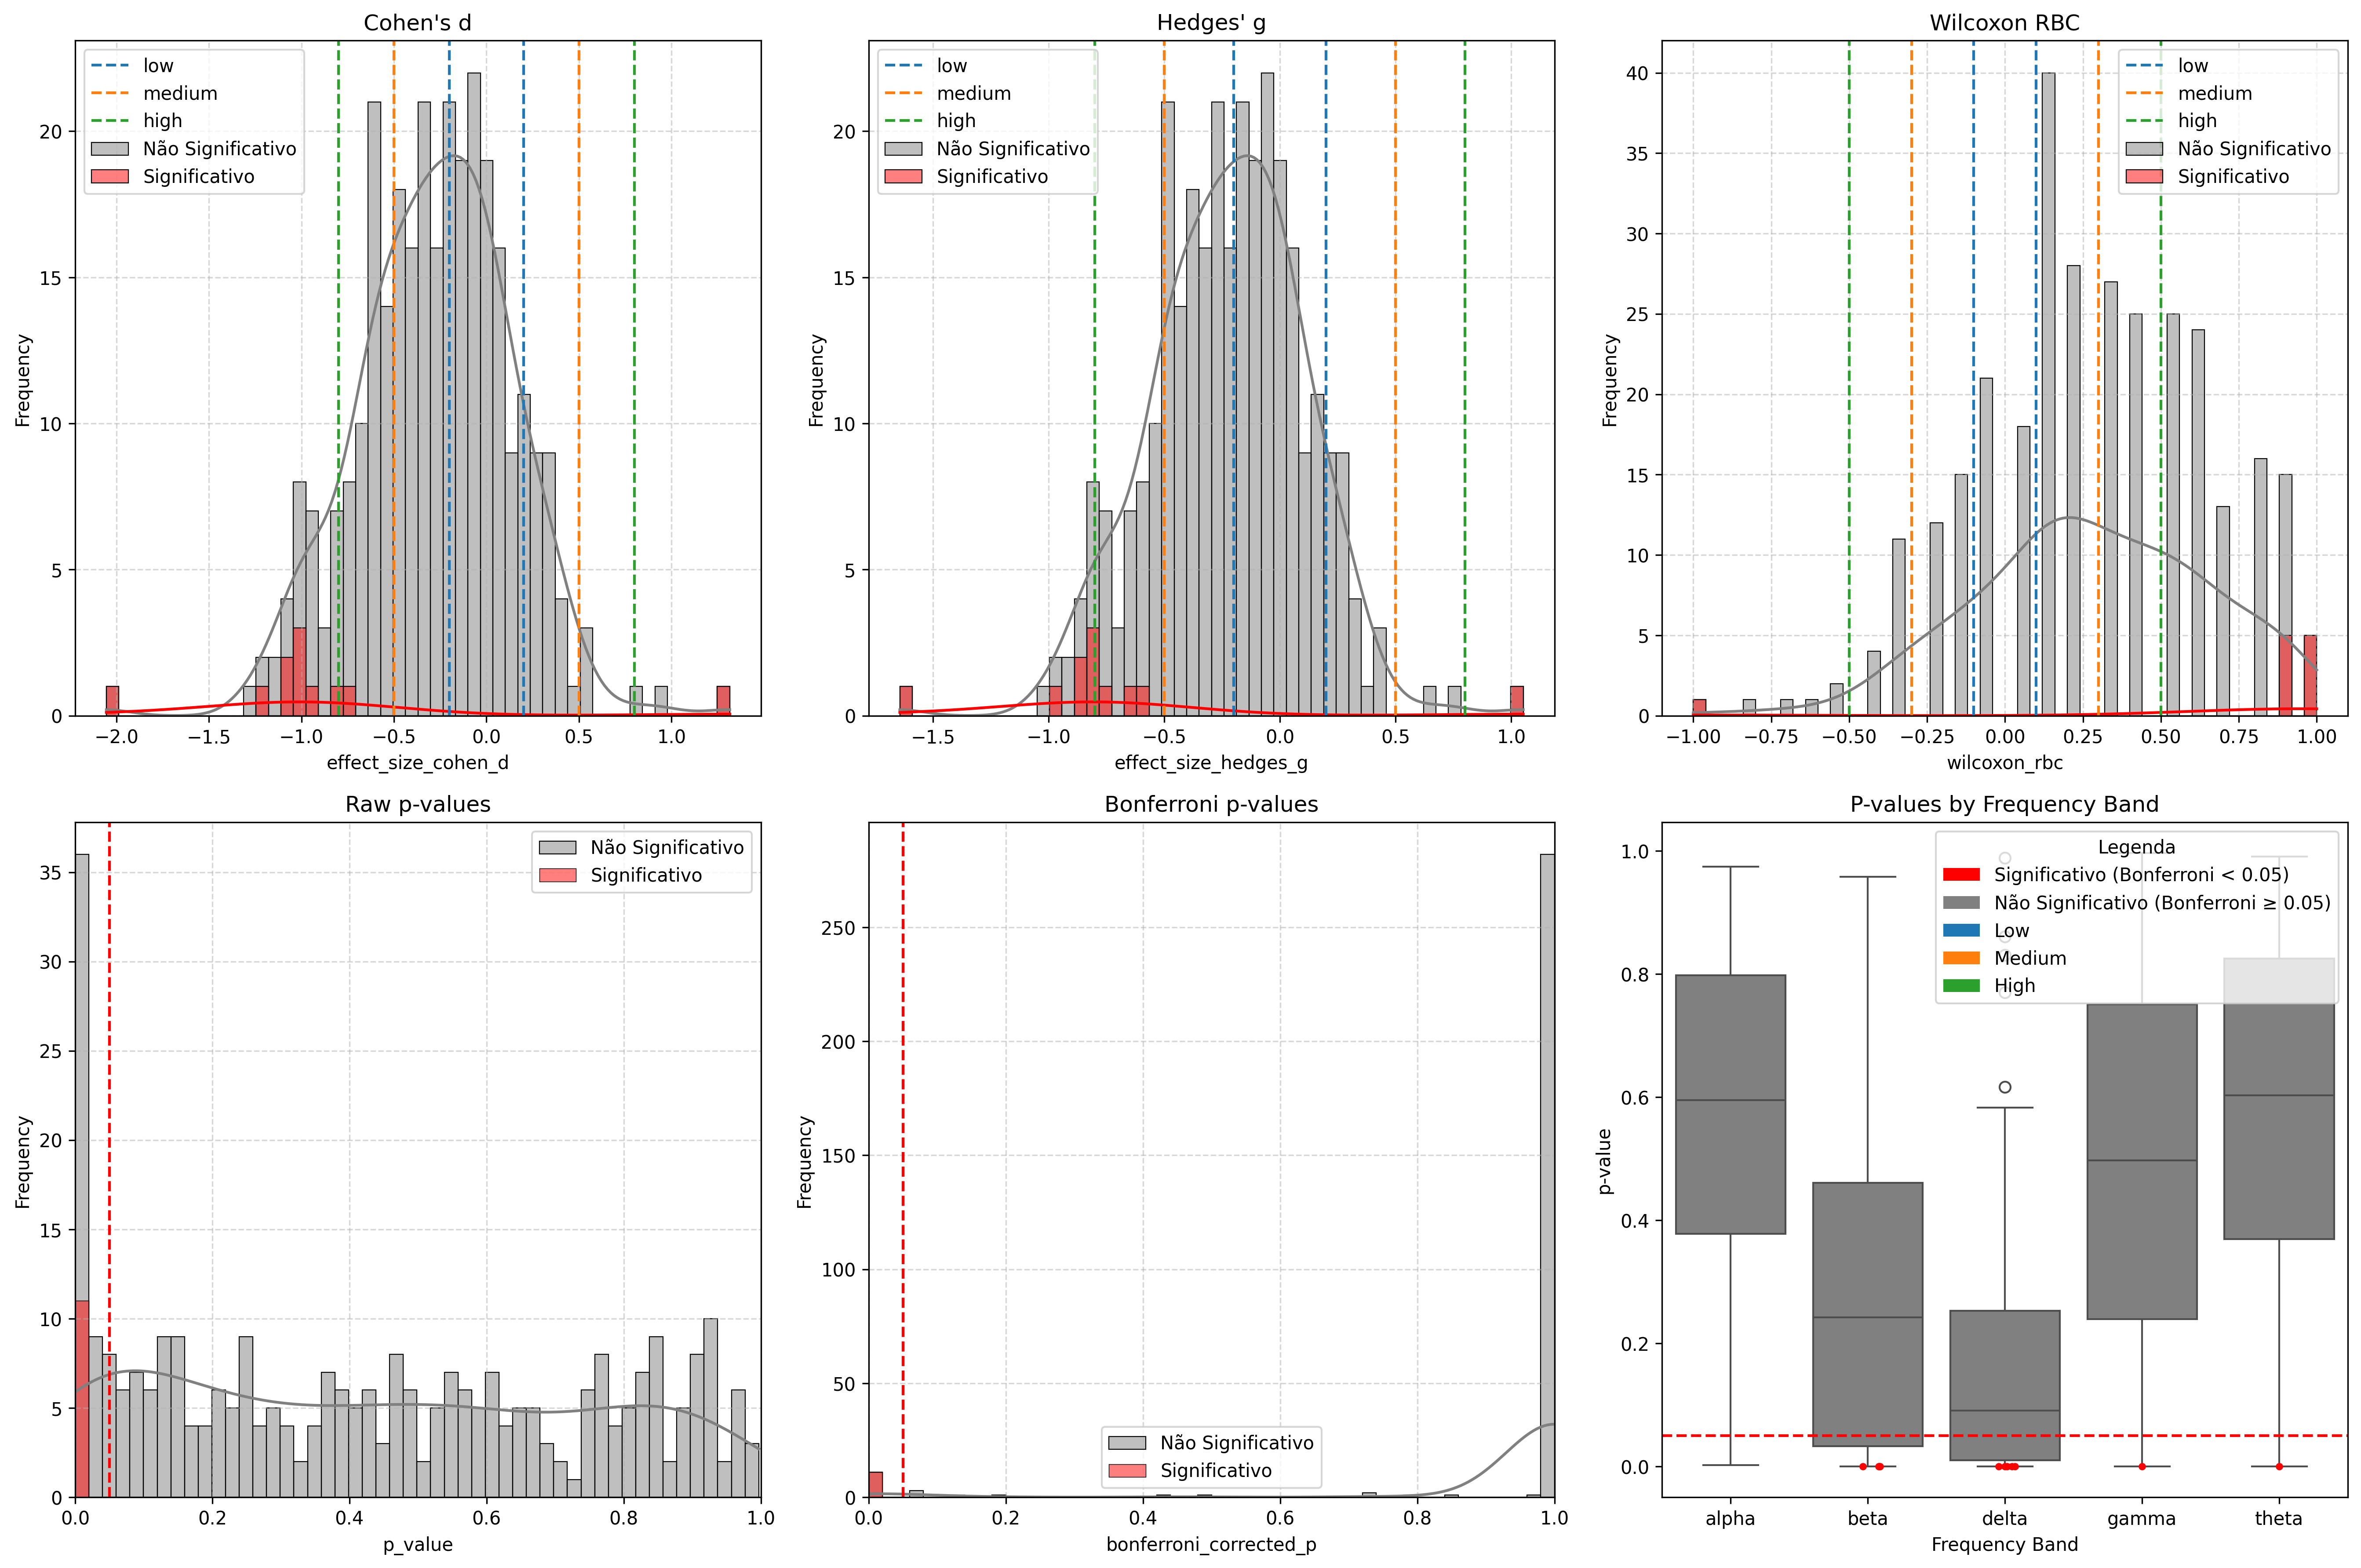
\includegraphics[width=0.45\textwidth]{figs/7_bootstrap_results_analysis/1_effect_size_histograms/Effect_Size_Histograms_CFPLM_EEGECG_Com_Outliers.png}
    }
    \caption[Distribuições de tamanhos de efeito e valores-p]{Distribuição das métricas de tamanho de efeito (\emph{Cohen's d}, \emph{Hedges' g} e \emph{Wilcoxon RBC}) e dos valores-p (brutos e corrigidos por Bonferroni) para PLI (EEG-EEG) e CF-PLM (EEG-ECG), em cenários com e sem outliers. O \emph{Wilcoxon RBC} e o p-valor corrigido por Bonferroni (vertical tracejada vermelha em $p=0.05$) são enfatizados como as métricas mais robustas para, respectivamente, o tamanho de efeito e a significância estatística.}
    \label{fig:effectsizehist_all}
\end{figure}

\subsection{Distribuição dos Tamanhos de Efeito}

\paragraph{Cohen's d e Hedges' g}
\begin{itemize}
    \item A maior parte dos valores concentra-se em torno de zero, indicando que, para a maioria dos pares, as diferenças entre \emph{cathodic} e \emph{sham} são pequenas ou não significativas.
    \item Valores significativos (barras vermelhas nos histogramas) tendem a se afastar de zero, sinalizando diferenças mais acentuadas. Por exemplo, \emph{Cohen's d} ou \emph{Hedges' g} acima de 0.5 (ou abaixo de -0.5) sugere um efeito moderado, e acima de 0.8 (ou abaixo de -0.8) indica um efeito alto.
    \item \emph{Hedges' g} difere de \emph{Cohen's d} por aplicar uma correção para tamanhos amostrais pequenos, mas ambas exibem comportamentos semelhantes nos histogramas.
\end{itemize}

\paragraph{Wilcoxon RBC (Rank-Biserial Correlation)}
\begin{itemize}
    \item O \emph{Wilcoxon RBC} é derivado do teste não paramétrico de Wilcoxon, refletindo a correlação de postos entre as condições (tipicamente variando de -1 a +1).
    \item Por não exigir pressupostos de normalidade, o RBC mostra-se mais robusto ao lidar com dados heterogêneos e eventuais outliers. 
    \item Valores acima de 0.3 ou abaixo de -0.3 sugerem efeito moderado; acima de 0.5 (ou abaixo de -0.5) indicam efeito alto. Quando se aproxima de ±1, as condições diferem de forma quase absoluta.
    \item Devido a essa robustez, o RBC será nosso principal indicador de tamanho de efeito nas análises subsequentes.
\end{itemize}


\subsection{Distribuição de p-valores (Brutos e Corrigidos)}

\begin{itemize}
    \item Os histogramas de valores-p brutos exibem forte concentração em torno de 1 (resultados não significativos) e uma cauda próxima de 0 (potenciais resultados significativos).
    \item Após a correção de Bonferroni (marcada pela linha vertical tracejada em $p=0.05$), muitos valores que eram marginalmente significativos são deslocados para a região de não significância, evidenciando o caráter conservador desta correção.
    \item Em virtude do elevado número de comparações, a adoção de um método rigoroso como o Bonferroni minimiza a probabilidade de falsos positivos. Por esse motivo, utilizamos o p-valor corrigido por Bonferroni como critério principal de significância.
\end{itemize}

\subsection{Comparação Entre Cenários (Com e Sem Outliers)}
\begin{itemize}
    \item \textbf{Diferenças Mínimas:} Em geral, a remoção de outliers reduz ligeiramente o número de casos significativos, mas não altera substancialmente a distribuição geral dos tamanhos de efeito e dos valores-p.
    \item \textbf{PLI (EEG-EEG):} Apresenta maior número de efeitos significativos (por exemplo, 378 vs. 363), enquanto o \emph{CF-PLM (EEG-ECG)} se mostra mais pontual (apenas 11 casos) em ambos os cenários, evidenciando que a sincronia cross-frequency entre EEG e ECG é mais específica.
    \item \textbf{Robustez do RBC e do Bonferroni:} Independentemente de manter ou remover outliers, as comparações que exibem \emph{Wilcoxon RBC} elevado e valores-p corrigidos abaixo de 0.05 são consideradas efeitos fortes e confiáveis, reforçando a relevância dessas duas métricas em nossas conclusões.
\end{itemize}

Em síntese, os histogramas de \emph{Wilcoxon RBC} (tamanho de efeito) e p-valores corrigidos por Bonferroni (significância estatística) demonstram claramente quais pares de canais se destacam por apresentarem diferenças robustas entre \emph{cathodic} e \emph{sham}. Embora \emph{Cohen's d} e \emph{Hedges' g} também sejam úteis para quantificar a magnitude do efeito, nossa análise dá ênfase ao RBC por ser não paramétrico e resiliente à heterogeneidade dos dados. Assim, estes resultados embasam as análises topográficas e de rede apresentadas nas seções seguintes.


\subsection{Comparação Entre Cenários (Com e Sem Outliers)}
\begin{itemize}
    \item \textbf{Redução de Casos Significativos:} Para o PLI em \texttt{EEG\_EEG}, por exemplo, temos 378 casos significantes ao manter os outliers e 363 após removê-los. A remoção de outliers atenua ligeiramente os valores extremos, reduzindo o número de pares que atingem significância, mas não altera drasticamente a distribuição geral.
    \item \textbf{Magnitude dos Efeitos:} Mesmo sem outliers, ainda há uma parcela considerável de pares exibindo \emph{Cohen's d} (ou \emph{Hedges' g}) em torno de 0.5 a 0.8 ou RBC acima de 0.3, sugerindo efeitos moderados a altos em alguns canais ou faixas de frequência.
    \item \textbf{CF-PLM em \texttt{EEG\_ECG}:} Observa-se um número bem menor de casos significativos (11 em ambos os cenários), o que indica que a sincronia entre EEG e ECG (medida pelo CF-PLM) é mais pontual e dependente de condições específicas, em contraste com a PLI \texttt{EEG\_EEG}, que registra maior número de efeitos estatisticamente relevantes.
\end{itemize}

\subsection{Conclusões Principais}
\begin{itemize}
    \item A maior parte dos dados concentra-se em torno de zero para todas as métricas, refletindo pequenas diferenças entre as condições, o que é coerente com métodos robustos de correção múltipla (p.\,ex.\ Bonferroni) e o grande número de comparações.
    \item Quando há significância estatística, os tamanhos de efeito se afastam notavelmente de zero (\emph{Cohen's d}, \emph{Hedges' g} ou RBC), sugerindo diferenças substanciais e possivelmente relevantes do ponto de vista neurofisiológico.
    \item O \emph{Wilcoxon RBC} se mostra particularmente robusto para capturar a direção e a magnitude das diferenças sem pressupor normalidade, razão pela qual será enfatizado nas próximas análises topográficas e de grafos de conectividade.
\end{itemize}

Assim, a análise dos histogramas de tamanho de efeito e valores-p fornece um panorama inicial: embora haja muitos casos não significativos, uma fração não desprezível apresenta efeitos moderados ou altos e valores-p corrigidos abaixo do limiar. Tais resultados embasam investigações posteriores, que buscarão caracterizar a localização e as faixas de frequência onde a \emph{neuromodulação} exerce impacto mais pronunciado.


\section{Análise de Rede para PLI (EEG-EEG)}
\label{sec:rede_pli_eeg}

Nesta seção, analisamos as redes de conexões significativas obtidas pela métrica PLI para pares EEG-EEG, segmentadas por bandas de frequência, considerando os cenários com e sem outliers. Em cada grafo, cada nó representa um canal EEG e o número exibido ao lado indica a quantidade de conexões significativas envolvendo aquele canal. As linhas conectando os nós correspondem aos pares significativos, onde as linhas vermelhas indicam valores de \emph{Wilcoxon RBC} tendendo a +1 (indicando conexões com efeitos extremamente fortes), enquanto linhas em azul indicariam valores próximos a -1 (não observados neste estudo).

A seguir, apresentamos os gráficos para cada banda de frequência.

\subsection{Cenário Sem Outliers}
\subsubsection{\texorpdfstring{Banda Delta (0.5--4\,Hz)}{Banda Delta (0.5-4 Hz)}}
\begin{figure}[htb]
  \centering
  \includegraphics[width=0.8\textwidth]{figs/7_bootstrap_results_analysis/2_network_graphs/PLI_EEG-EEG_Sem_Outliers/Banda_Delta_(0.5_a_4_Hz)_-_Análise_de_Rede_-_PLI_EEG-EEG_Sem_Outliers.png}
  \caption{Rede de conexões significativas na banda Delta (0.5--4\,Hz) para PLI (EEG-EEG) sem outliers. A rede é esparsa, com poucas conexões, o que sugere que a sincronização nessa faixa é limitada e pontual.}
  \label{fig:rede_pli_delta_sem}
\end{figure}

\subsubsection{\texorpdfstring{Banda Theta (4--8\,Hz)}{Banda Theta (4-8 Hz)}}
\begin{figure}[htb]
  \centering
  \includegraphics[width=0.8\textwidth]{figs/7_bootstrap_results_analysis/2_network_graphs/PLI_EEG-EEG_Sem_Outliers/Banda_Theta_(4_Hz_a_8_Hz)_-_Análise_de_Rede_-_PLI_EEG-EEG_Sem_Outliers.png}
  \caption{Rede de conexões significativas na banda Theta (4--8\,Hz) para PLI (EEG-EEG) sem outliers. A conectividade é moderada, com alguns canais exibindo um número elevado de conexões, indicando sua importância na sincronização nesta faixa.}
  \label{fig:rede_pli_theta_sem}
\end{figure}

\subsubsection{\texorpdfstring{Banda Alpha (8--13\,Hz)}{Banda Alpha (8-13 Hz)}}
\begin{figure}[htb]
  \centering
  \includegraphics[width=0.8\textwidth]{figs/7_bootstrap_results_analysis/2_network_graphs/PLI_EEG-EEG_Sem_Outliers/Banda_Alpha_(8_Hz_a_13_Hz)_-_Análise_de_Rede_-_PLI_EEG-EEG_Sem_Outliers.png}
  \caption{Rede de conexões significativas na banda Alpha (8--13\,Hz) para PLI (EEG-EEG) sem outliers. Observa-se uma rede densa com um núcleo central de canais altamente conectados, sugerindo uma forte sincronização nesta banda.}
  \label{fig:rede_pli_alpha_sem}
\end{figure}

\subsubsection{\texorpdfstring{Banda Beta (13--30\,Hz)}{Banda Beta (13-30 Hz)}}
\begin{figure}[htb]
  \centering
  \includegraphics[width=0.8\textwidth]{figs/7_bootstrap_results_analysis/2_network_graphs/PLI_EEG-EEG_Sem_Outliers/Banda_Beta_(13_Hz_a_30_Hz)_-_Análise_de_Rede_-_PLI_EEG-EEG_Sem_Outliers.png}
  \caption{Rede de conexões significativas na banda Beta (13--30\,Hz) para PLI (EEG-EEG) sem outliers. A rede apresenta conectividade intermediária, com uma distribuição relativamente homogênea das conexões entre os canais.}
  \label{fig:rede_pli_beta_sem}
\end{figure}

\subsubsection{\texorpdfstring{Banda Gamma (30--60\,Hz)}{Banda Gamma (30-60 Hz)}}
\begin{figure}[htb]
  \centering
  \includegraphics[width=0.8\textwidth]{figs/7_bootstrap_results_analysis/2_network_graphs/PLI_EEG-EEG_Sem_Outliers/Banda_Gamma_(30_Hz_a_60_Hz)_-_Análise_de_Rede_-_PLI_EEG-EEG_Sem_Outliers.png}
  \caption{Rede de conexões significativas na banda Gamma (30--60\,Hz) para PLI (EEG-EEG) sem outliers. A rede é mais esparsa, mas destaca alguns pares de canais com conexões extremamente robustas.}
  \label{fig:rede_pli_gamma_sem}
\end{figure}

\subsection{Cenário Com Outliers}
\subsubsection{\texorpdfstring{Banda Delta (0.5--4\,Hz)}{Banda Delta (0.5-4 Hz)}}
\begin{figure}[htb]
  \centering
  \includegraphics[width=0.8\textwidth]{figs/7_bootstrap_results_analysis/2_network_graphs/PLI_EEG-EEG_Com_Outliers/Banda_Delta_(0.5_a_4_Hz)_-_Análise_de_Rede_-_PLI_EEG-EEG_Com_Outliers.png}
  \caption{Rede de conexões significativas na banda Delta (0.5--4\,Hz) para PLI (EEG-EEG) com outliers mantidos. A estrutura é similar à observada sem outliers, com poucas conexões significativas.}
  \label{fig:rede_pli_delta_com}
\end{figure}

\subsubsection{\texorpdfstring{Banda Theta (4--8\,Hz)}{Banda Theta (4-8 Hz)}}
\begin{figure}[htb]
  \centering
  \includegraphics[width=0.8\textwidth]{figs/7_bootstrap_results_analysis/2_network_graphs/PLI_EEG-EEG_Com_Outliers/Banda_Theta_(4_Hz_a_8_Hz)_-_Análise_de_Rede_-_PLI_EEG-EEG_Com_Outliers.png}
  \caption{Rede de conexões significativas na banda Theta (4--8\,Hz) para PLI (EEG-EEG) com outliers mantidos. A conectividade moderada e os canais com alta centralidade se mantêm, confirmando a robustez dos efeitos.}
  \label{fig:rede_pli_theta_com}
\end{figure}

\subsubsection{\texorpdfstring{Banda Alpha (8--13\,Hz)}{Banda Alpha (8-13 Hz)}}
\begin{figure}[htb]
  \centering
  \includegraphics[width=0.8\textwidth]{figs/7_bootstrap_results_analysis/2_network_graphs/PLI_EEG-EEG_Com_Outliers/Banda_Alpha_(8_Hz_a_13_Hz)_-_Análise_de_Rede_-_PLI_EEG-EEG_Com_Outliers.png}
  \caption{Rede de conexões significativas na banda Alpha (8--13\,Hz) para PLI (EEG-EEG) com outliers mantidos. A rede densa e o núcleo central de canais altamente conectados permanecem, demonstrando uma forte sincronização, similar à observada sem outliers.}
  \label{fig:rede_pli_alpha_com}
\end{figure}

\subsubsection{\texorpdfstring{Banda Beta (13--30\,Hz)}{Banda Beta (13-30 Hz)}}
\begin{figure}[htb]
  \centering
  \includegraphics[width=0.8\textwidth]{figs/7_bootstrap_results_analysis/2_network_graphs/PLI_EEG-EEG_Com_Outliers/Banda_Beta_(13_Hz_a_30_Hz)_-_Análise_de_Rede_-_PLI_EEG-EEG_Com_Outliers.png}
  \caption{Rede de conexões significativas na banda Beta (13--30\,Hz) para PLI (EEG-EEG) com outliers mantidos. A distribuição das conexões é semelhante à observada no cenário sem outliers, evidenciando uma conectividade intermediária.}
  \label{fig:rede_pli_beta_com}
\end{figure}

\subsubsection{\texorpdfstring{Banda Gamma (30--60\,Hz)}{Banda Gamma (30-60 Hz)}}
\begin{figure}[htb]
  \centering
  \includegraphics[width=0.8\textwidth]{figs/7_bootstrap_results_analysis/2_network_graphs/PLI_EEG-EEG_Com_Outliers/Banda_Gamma_(30_Hz_a_60_Hz)_-_Análise_de_Rede_-_PLI_EEG-EEG_Com_Outliers.png}
  \caption{Rede de conexões significativas na banda Gamma (30--60\,Hz) para PLI (EEG-EEG) com outliers mantidos. Mesmo com a presença de outliers, a rede se mantém esparsa, destacando os pares de canais com conexões robustas.}
  \label{fig:rede_pli_gamma_com}
\end{figure}

\subsection{Análise Comparativa dos Cenários}
A comparação entre os cenários com e sem outliers para a métrica PLI em pares EEG-EEG evidencia que:
\begin{itemize}
    \item \textbf{Topologia Geral Inalterada:} A estrutura das redes – identificada por canais com maior centralidade e o padrão de conexões – permanece praticamente a mesma em ambos os cenários.
    \item \textbf{Número de Conexões:} Há uma ligeira redução no número de conexões significativas quando os outliers são removidos (por exemplo, 378 casos com outliers versus 363 sem outliers), o que é esperado, pois a remoção de valores extremos pode atenuar alguns efeitos marginais.
    \item \textbf{Robustez dos Efeitos:} Os pares com \emph{Wilcoxon RBC} de +1, indicados pelas linhas vermelhas, persistem em ambos os cenários, reforçando a confiabilidade dos efeitos encontrados.
\end{itemize}

Essas observações corroboram a robustez da análise PLI, demonstrando que, embora a remoção de outliers reduza ligeiramente o número de conexões, a topologia e a intensidade dos efeitos permanecem consistentes.

\section{Análise de Rede para CF-PLM (EEG-ECG, Cross-frequency)}
\label{sec:rede_cfplm_eeg_ecg}

Nesta seção, avaliamos as redes de conectividade entre sinais de EEG e ECG obtidas pela métrica CF-PLM, que quantifica a sincronização entre frequências distintas (cross-frequency). Em cada gráfico, os nós representam os canais (tanto os canais EEG quanto o canal ECG) e o número exibido ao lado de cada nó indica a quantidade de conexões significativas envolvendo aquele canal. As linhas que conectam os nós representam os pares significativos; neste estudo, os casos significativos exibem \emph{Wilcoxon RBC} de +1, o que denota efeitos extremamente robustos (não foram observados casos com valores próximos a -1).

Observamos que, para CF-PLM, o número total de pares significativos é idêntico (11 casos) em ambos os cenários, indicando que os efeitos cross-frequency identificados são altamente robustos e não dependem da presença de outliers.

\subsection{Cenário Sem Outliers}
\subsubsection{\texorpdfstring{Banda Delta (0.5--4\,Hz)}{Banda Delta (0.5-4 Hz)}}
\begin{figure}[htb]
  \centering
  \includegraphics[width=0.8\textwidth]{figs/7_bootstrap_results_analysis/2_network_graphs/CF-PLM_EEG-ECG_Sem_Outliers/Banda_Delta_(0.5_a_4_Hz)_-_Análise_de_Rede_-_CF-PLM_EEG-ECG_Sem_Outliers.png}
  \caption{Rede CF-PLM na banda Delta (0.5--4\,Hz) para EEG-ECG sem outliers. A rede é bastante esparsa, indicando que a sincronização cross-frequency nesta faixa ocorre de forma pontual e em poucos pares de canais.}
  \label{fig:rede_cfplm_delta_sem}
\end{figure}

\subsubsection{\texorpdfstring{Banda Theta (4--8\,Hz)}{Banda Theta (4-8 Hz)}}
\begin{figure}[htb]
  \centering
  \includegraphics[width=0.8\textwidth]{figs/7_bootstrap_results_analysis/2_network_graphs/CF-PLM_EEG-ECG_Sem_Outliers/Banda_Theta_(4_Hz_a_8_Hz)_-_Análise_de_Rede_-_CF-PLM_EEG-ECG_Sem_Outliers.png}
  \caption{Rede CF-PLM na banda Theta (4--8\,Hz) para EEG-ECG sem outliers. A conectividade é moderada, com alguns canais apresentando maior número de conexões significativas, sugerindo que certos canais desempenham um papel crucial na integração cross-frequency nesta faixa.}
  \label{fig:rede_cfplm_theta_sem}
\end{figure}

\subsubsection{\texorpdfstring{Banda Alpha (8--13\,Hz)}{Banda Alpha (8-13 Hz)}}
\begin{figure}[htb]
  \centering
  \includegraphics[width=0.8\textwidth]{figs/7_bootstrap_results_analysis/2_network_graphs/CF-PLM_EEG-ECG_Sem_Outliers/Banda_Alpha_(8_Hz_a_13_Hz)_-_Análise_de_Rede_-_CF-PLM_EEG-ECG_Sem_Outliers.png}
  \caption{Rede CF-PLM na banda Alpha (8--13\,Hz) para EEG-ECG sem outliers. A rede apresenta conexões pontuais entre canais EEG e ECG, evidenciando a presença de sincronização cross-frequency específica nessa faixa.}
  \label{fig:rede_cfplm_alpha_sem}
\end{figure}

\subsubsection{\texorpdfstring{Banda Beta (13--30\,Hz)}{Banda Beta (13-30 Hz)}}
\begin{figure}[htb]
  \centering
  \includegraphics[width=0.8\textwidth]{figs/7_bootstrap_results_analysis/2_network_graphs/CF-PLM_EEG-ECG_Sem_Outliers/Banda_Beta_(13_Hz_a_30_Hz)_-_Análise_de_Rede_-_CF-PLM_EEG-ECG_Sem_Outliers.png}
  \caption{Rede CF-PLM na banda Beta (13--30\,Hz) para EEG-ECG sem outliers. Apesar da rede ser relativamente esparsa, os pares significativos indicam uma forte sincronização entre os canais, refletindo um efeito robusto nessa faixa.}
  \label{fig:rede_cfplm_beta_sem}
\end{figure}

\subsubsection{\texorpdfstring{Banda Gamma (30--60\,Hz)}{Banda Gamma (30-60 Hz)}}
\begin{figure}[htb]
  \centering
  \includegraphics[width=0.8\textwidth]{figs/7_bootstrap_results_analysis/2_network_graphs/CF-PLM_EEG-ECG_Sem_Outliers/Banda_Gamma_(30_Hz_a_60_Hz)_-_Análise_de_Rede_-_CF-PLM_EEG-ECG_Sem_Outliers.png}
  \caption{Rede CF-PLM na banda Gamma (30--60\,Hz) para EEG-ECG sem outliers. A rede destaca alguns pares com conexões extremamente robustas, embora a conectividade global seja pontual.}
  \label{fig:rede_cfplm_gamma_sem}
\end{figure}

\subsection{Cenário Com Outliers}
\subsubsection{\texorpdfstring{Banda Delta (0.5--4\,Hz)}{Banda Delta (0.5-4 Hz)}}
\begin{figure}[htb]
  \centering
  \includegraphics[width=0.8\textwidth]{figs/7_bootstrap_results_analysis/2_network_graphs/CF-PLM_EEG-ECG_Com_Outliers/Banda_Delta_(0.5_a_4_Hz)_-_Análise_de_Rede_-_CF-PLM_EEG-ECG_Com_Outliers.png}
  \caption{Rede CF-PLM na banda Delta (0.5--4\,Hz) para EEG-ECG com outliers. A estrutura da rede é idêntica à observada sem outliers, evidenciando a estabilidade dos efeitos cross-frequency nesta faixa.}
  \label{fig:rede_cfplm_delta_com}
\end{figure}

\subsubsection{\texorpdfstring{Banda Theta (4--8\,Hz)}{Banda Theta (4-8 Hz)}}
\begin{figure}[htb]
  \centering
  \includegraphics[width=0.8\textwidth]{figs/7_bootstrap_results_analysis/2_network_graphs/CF-PLM_EEG-ECG_Com_Outliers/Banda_Theta_(4_Hz_a_8_Hz)_-_Análise_de_Rede_-_CF-PLM_EEG-ECG_Com_Outliers.png}
  \caption{Rede CF-PLM na banda Theta (4--8\,Hz) para EEG-ECG com outliers. A conectividade e a distribuição dos nós permanecem semelhantes às observadas no cenário sem outliers.}
  \label{fig:rede_cfplm_theta_com}
\end{figure}

\subsubsection{\texorpdfstring{Banda Alpha (8--13\,Hz)}{Banda Alpha (8-13 Hz)}}
\begin{figure}[htb]
  \centering
  \includegraphics[width=0.8\textwidth]{figs/7_bootstrap_results_analysis/2_network_graphs/CF-PLM_EEG-ECG_Com_Outliers/Banda_Alpha_(8_Hz_a_13_Hz)_-_Análise_de_Rede_-_CF-PLM_EEG-ECG_Com_Outliers.png}
  \caption{Rede CF-PLM na banda Alpha (8--13\,Hz) para EEG-ECG com outliers. A topologia da rede é idêntica à observada sem outliers, demonstrando que os efeitos robustos não são afetados pela presença de valores extremos.}
  \label{fig:rede_cfplm_alpha_com}
\end{figure}

\subsubsection{\texorpdfstring{Banda Beta (13--30\,Hz)}{Banda Beta (13-30 Hz)}}
\begin{figure}[htb]
  \centering
  \includegraphics[width=0.8\textwidth]{figs/7_bootstrap_results_analysis/2_network_graphs/CF-PLM_EEG-ECG_Com_Outliers/Banda_Beta_(13_Hz_a_30_Hz)_-_Análise_de_Rede_-_CF-PLM_EEG-ECG_Com_Outliers.png}
  \caption{Rede CF-PLM na banda Beta (13--30\,Hz) para EEG-ECG com outliers. A rede apresenta uma conectividade robusta e a mesma topologia dos gráficos sem outliers, indicando que os valores extremos não alteram significativamente os efeitos identificados.}
  \label{fig:rede_cfplm_beta_com}
\end{figure}

\subsubsection{\texorpdfstring{Banda Gamma (30--60\,Hz)}{Banda Gamma (30-60 Hz)}}
\begin{figure}[htb]
  \centering
  \includegraphics[width=0.8\textwidth]{figs/7_bootstrap_results_analysis/2_network_graphs/CF-PLM_EEG-ECG_Com_Outliers/Banda_Gamma_(30_Hz_a_60_Hz)_-_Análise_de_Rede_-_CF-PLM_EEG-ECG_Com_Outliers.png}
  \caption{Rede CF-PLM na banda Gamma (30--60\,Hz) para EEG-ECG com outliers. A rede exibe os mesmos pares robustos de conexão (RBC = +1) observados sem outliers, confirmando a estabilidade dos efeitos cross-frequency na faixa de alta frequência.}
  \label{fig:rede_cfplm_gamma_com}
\end{figure}

\subsection{Comparação Geral entre Cenários para CF-PLM}
Ao comparar os resultados dos cenários com e sem outliers para CF-PLM (EEG-ECG), observamos:
\begin{itemize}
    \item \textbf{Topologia Consistente:} A estrutura das redes – ou seja, quais canais se conectam e a contagem de conexões – é praticamente idêntica em ambos os cenários, para todas as bandas de frequência.
    \item \textbf{Número de Conexões Inalterado:} O número total de pares significativos (11 casos) permanece constante, evidenciando que os efeitos cross-frequency são robustos e não dependem da remoção de outliers.
    \item \textbf{Robustez dos Efeitos:} Todos os pares significativos exibem \emph{Wilcoxon RBC} de +1, demonstrando que, independentemente da presença de outliers, os efeitos são extremamente fortes.
\end{itemize}

Essas análises confirmam a estabilidade e robustez dos efeitos cross-frequency medidos pelo CF-PLM para a interação entre EEG e ECG, fornecendo uma base sólida para investigações futuras sobre a integração dos sistemas neural e cardíaco.